\documentclass[10pt,conference,compsocconf]{IEEEtran}

\usepackage{hyperref}
\usepackage{graphicx}	% For figure environment
\usepackage{amsmath,amssymb}
\usepackage{booktabs}


\begin{document}
\title{Predicting Coronary Heart Disease from Survey Data with Linear Models}

\author{
  Chiara Candiotti, Ittirath Wiwatwanont, Mercy Eze\\
  \textit{CS-433 Machine Learning, EPFL, Switzerland}\\
  Code: \url{https://github.com/Candicci/ML_Project_HeartAttack}
}

\maketitle

\begin{abstract}
  We predict whether a person has been diagnosed with coronary heart disease
  (MICHD) from 321 health and lifestyle features of the BRFSS telephone survey.
  Early detection of cardiovascular disease matters, but the task is hard: only
  8.8\% of the respondents are positive and about 45\% of the feature values are
  missing. We implement six linear methods from scratch (least squares, ridge,
  linear regression with GD and SGD, and logistic regression with and without
  regularization) and compare them in one shared pipeline. With the default
  decision cutoff all of them reach an F1 score of at most 0.18. Tuning the cutoff
  on a validation set raises it to 0.39--0.41 for every method, which matters much
  more than the choice of model. Our logistic regression scores F1 = 0.416 on the
  competition test set.
\end{abstract}

\section{Introduction}

The dataset contains 328,135 labelled respondents (321 features) and 109,379
unlabelled ones for the competition. The label is $+1$ if the respondent reported
MICHD (heart attack or angina) and $-1$ otherwise. Because positives are rare, a
classifier that always predicts $-1$ already reaches 91\% accuracy, so we use the F1
score of the positive class as the main metric.

Our contributions are: (i) correct implementations of the six required methods,
all trained and tuned with the same preprocessing and protocol; (ii) an ablation
showing that the decision cutoff is the most important choice for this imbalanced
problem; and (iii) evidence that all linear models perform alike once the cutoff
is tuned, and that none of them overfits.

\section{Models and Methods}
\label{sec:methods}

\subsection{Data and preprocessing}
We split the labelled data at random (seed 42) into train / validation / test sets
of 80/10/10\% (262,508 / 32,813 / 32,814 rows). The positive rate is 8.8--8.9\% in
each split. All statistics are computed on the train split only. We drop the 6
columns that are constant or entirely missing, standardize each remaining column to
zero mean and unit variance, replace missing values by 0 (i.e.\ the train mean), and
add a bias column. This gives $D = 316$ inputs. The same transformation is applied
to the validation, test and competition sets. Standardization is essential: some
raw columns reach $\sim 10^9$, which makes the sigmoid overflow.

\subsection{Models}
Let $\mathbf{x}_n \in \mathbb{R}^D$ be the preprocessed features and $N$ the number
of training rows. The linear-regression methods use labels $y_n \in \{-1, 1\}$ and
the MSE loss; the logistic methods use $y_n \in \{0, 1\}$ and the negative
log-likelihood:
\begin{align*}
  L_{\text{MSE}}(\mathbf{w}) &= \tfrac{1}{2N} \textstyle\sum_n (y_n - \mathbf{x}_n^\top \mathbf{w})^2, \\
  L_{\text{NLL}}(\mathbf{w}) &= \tfrac{1}{N} \textstyle\sum_n \big[\log(1 + e^{\mathbf{x}_n^\top \mathbf{w}}) - y_n \mathbf{x}_n^\top \mathbf{w}\big].
\end{align*}
\emph{Least squares} solves the normal equations $X^\top X \mathbf{w} = X^\top \mathbf{y}$
and \emph{ridge regression} solves $(X^\top X + 2N\lambda I)\mathbf{w} = X^\top \mathbf{y}$.
\emph{GD} and \emph{SGD} (one random sample per step) minimize $L_{\text{MSE}}$.
\emph{Logistic regression} runs gradient descent on $L_{\text{NLL}}$, and the
\emph{regularized} version adds $\lambda \|\mathbf{w}\|^2$ to the objective. We
compute $\log(1 + e^z)$ with \texttt{np.logaddexp} so that it cannot overflow. All
methods predict $\hat y = +1$ if $\mathbf{x}^\top \mathbf{w} \ge t$ and $-1$ otherwise,
with cutoff $t$.

\subsection{Training and evaluation protocol}
All iterative methods start from $\mathbf{w}_0 = \mathbf{0}$. GD and both logistic
methods run 200 full-gradient iterations. SGD runs 10 epochs of $N$ single-sample
steps. We sweep the step size $\gamma$ on log grids: $\{10^{-3}, \dots, 10^{-1}\}$ for
GD, $\{10^{-4}, \dots, 3\cdot10^{-3}\}$ for SGD and $\{10^{-2}, \dots, 1\}$ for
logistic regression. For ridge we sweep 17 values $\lambda \in [10^{-8}, 1]$, and for
regularized logistic regression $\lambda \in \{10^{-5}, \dots, 10^{-1}\}$, using the
best logistic $\gamma$. Each hyperparameter is chosen by the lowest
\emph{validation} loss. We obtain loss curves at no extra cost by running the
methods in chunks of iterations and restarting each chunk from the previous
$\mathbf{w}$; this gives exactly the same weights as a single run.

The cutoff $t$ is then tuned per method on the validation set: we try 200
quantiles of the validation scores $\mathbf{x}^\top \mathbf{w}$ and keep the one
with the highest F1. The final method is the one with the best validation F1. The
test split is used only to report results. The notebook \texttt{run.ipynb}
reproduces all numbers and the submitted predictions.

\section{Results}

\begin{table}[tbp]
  \centering
  \small
  \setlength{\tabcolsep}{3pt}
  \begin{tabular}{@{}llccc@{}}
    \toprule
    Method & Hyperparameters & Acc. & F1 ($t=0$) & F1 (tuned $t$) \\
    \midrule
    GD            & $\gamma = 0.03$                 & 0.860 & 0.004 & 0.400 \\
    SGD           & $\gamma = 10^{-4}$              & 0.865 & 0.007 & 0.386 \\
    Least squares & --                              & 0.864 & 0.017 & 0.411 \\
    Ridge         & $\lambda = 3\cdot10^{-6}$       & 0.862 & 0.016 & 0.412 \\
    Logistic      & $\gamma = 1$                    & 0.858 & 0.183 & \textbf{0.413} \\
    Reg.\ logistic & $\gamma = 1$, $\lambda = 10^{-5}$ & 0.851 & 0.183 & 0.412 \\
    \bottomrule
  \end{tabular}
  \caption{Results on our local test split (32,814 rows). Accuracy is at the
    tuned cutoff. Logistic regression (cutoff $t = -1.48$) was selected on
    validation F1 (0.417) and scored F1 = 0.416, accuracy = 0.860 on the
    competition test set.}
  \vspace{-3mm}
  \label{tab:results}
\end{table}

\begin{figure}[tbp]
  \centering
  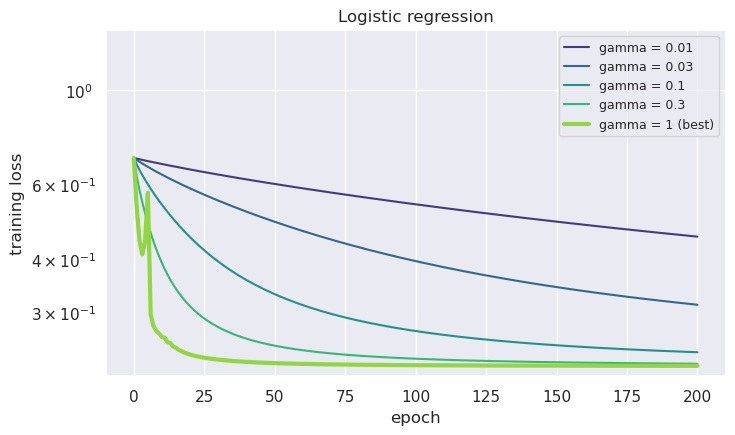
\includegraphics[width=\columnwidth]{fig_logistic_sweep}
  \vspace{-6mm}
  \caption{Training loss ($L_{\text{NLL}}$, log scale) of logistic regression for
    each step size $\gamma$; one epoch is one full-gradient iteration.}
  \vspace{-3mm}
  \label{fig:logistic-sweep}
\end{figure}

Table~\ref{tab:results} summarizes the test results. \textbf{The cutoff is the
dominant factor.} With $t = 0$ the linear-regression models almost never predict
$+1$ (F1 $\le 0.02$), and the logistic models only reach F1 = 0.18. Tuning $t$
raises F1 by 0.23 (logistic) to 0.40 (GD). All tuned cutoffs are negative ($\approx
-0.57$ for MSE scores, $-1.48$ to $-1.54$ for logistic scores), meaning that many more
people must be flagged than with the default cutoff. The price is a small loss in
accuracy: 0.85--0.87, compared with 0.91 for always predicting $-1$. After tuning, the six methods lie within 0.03 F1 of each
other; logistic regression wins narrowly and generalizes to the competition test
set (0.416 against 0.413 locally).

\textbf{Step size.} Figure~\ref{fig:logistic-sweep} shows that small step sizes
converge slowly, while $\gamma = 1$ converges fastest after a short initial
instability. For the MSE methods, too large a step size diverges: GD with
$\gamma = 0.1$ and SGD with $\gamma \ge 3\cdot10^{-4}$ (the training loss reaches
$10^{139}$ and then \texttt{inf}). SGD needs a much smaller $\gamma$ because each
step is based on a single noisy sample.

\textbf{Regularization} has almost no effect. Ridge validation loss is flat for
$\lambda \le 10^{-3}$, and the best regularized logistic model uses the smallest
$\lambda$ in the grid. With $N \approx 262{,}000 \gg D = 316$ there is little
variance to reduce, and train and test F1 differ by at most 0.007 for every model.

\textbf{Least squares and conditioning.} The design matrix has rank 310 of 316
(linearly dependent columns), so $X^\top X$ is singular
($\text{cond} \approx 9\cdot10^{18}$). On the full data the solver still returns
usable weights, but in an early experiment on a 5,250-row subsample the same
solver gave a validation MSE of $4\cdot10^4$. Ridge with any $\lambda > 0$ removes
this problem.

\section{Discussion}

Train and test performance are almost identical, so our models \emph{underfit}
rather than overfit: a linear decision rule on the raw survey codes is the
limiting factor, not the amount of data or the regularization. This is consistent
with the six very different training methods converging to the same F1. Two
weaknesses of our setup point to the next steps. First, many BRFSS features are
categorical codes (e.g.\ 7/9 for ``don't know/refused'', 88 for ``none'') that we
treat as numbers; one-hot encoding or recoding these values, together with
missing-value indicators, should give the linear models more useful features.
Second, we use a single train/validation/test split. The splits are large (about
33,000 rows each) and validation and test F1 agree, but $k$-fold cross-validation
would give the standard deviation of our estimates. Finally, the selected
$\gamma = 1$ lies at the edge of its grid, so a wider sweep or more iterations could
still give a small gain.

\section{Summary}

We implemented and compared six linear methods for predicting coronary heart disease
on a large, imbalanced and incomplete survey dataset. With careful standardization
all methods train stably, and tuning the decision cutoff on a validation set is by
far the most effective change, raising F1 from at most 0.18 to about 0.41. Our
selected logistic regression model reaches F1 = 0.416 and accuracy = 0.860 on the
competition test set.

\end{document}
